\chapter{Исследовательская часть}

\section{Среда для тестирования}

Для тестирования разработанного алгоритма применялась облачная платформа Google Colab, не требующая установки ПО на локальный компьютер.

% 
\
\section{Анализ результатов социологического исследования}

\begin{figure}
	\begin{center}
		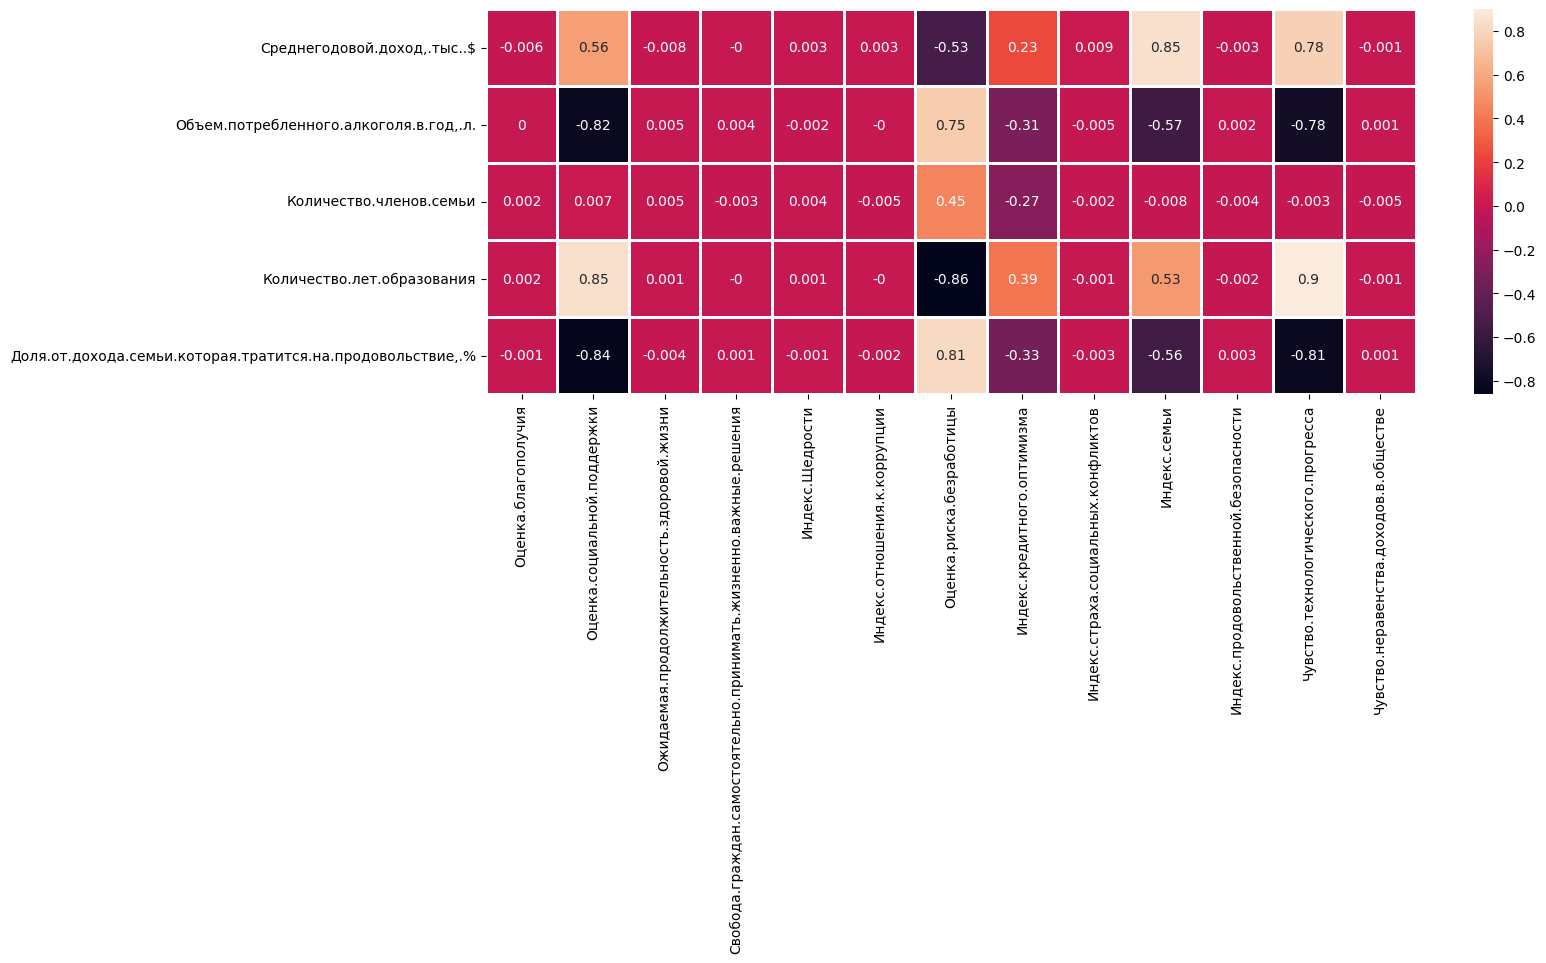
\includegraphics[width=\textwidth]{images/1.png}
	\end{center}
	\caption{Корреляция признаков причины и признаков состояния}
	\label{img:1}
\end{figure}

\begin{figure}
	\begin{center}
		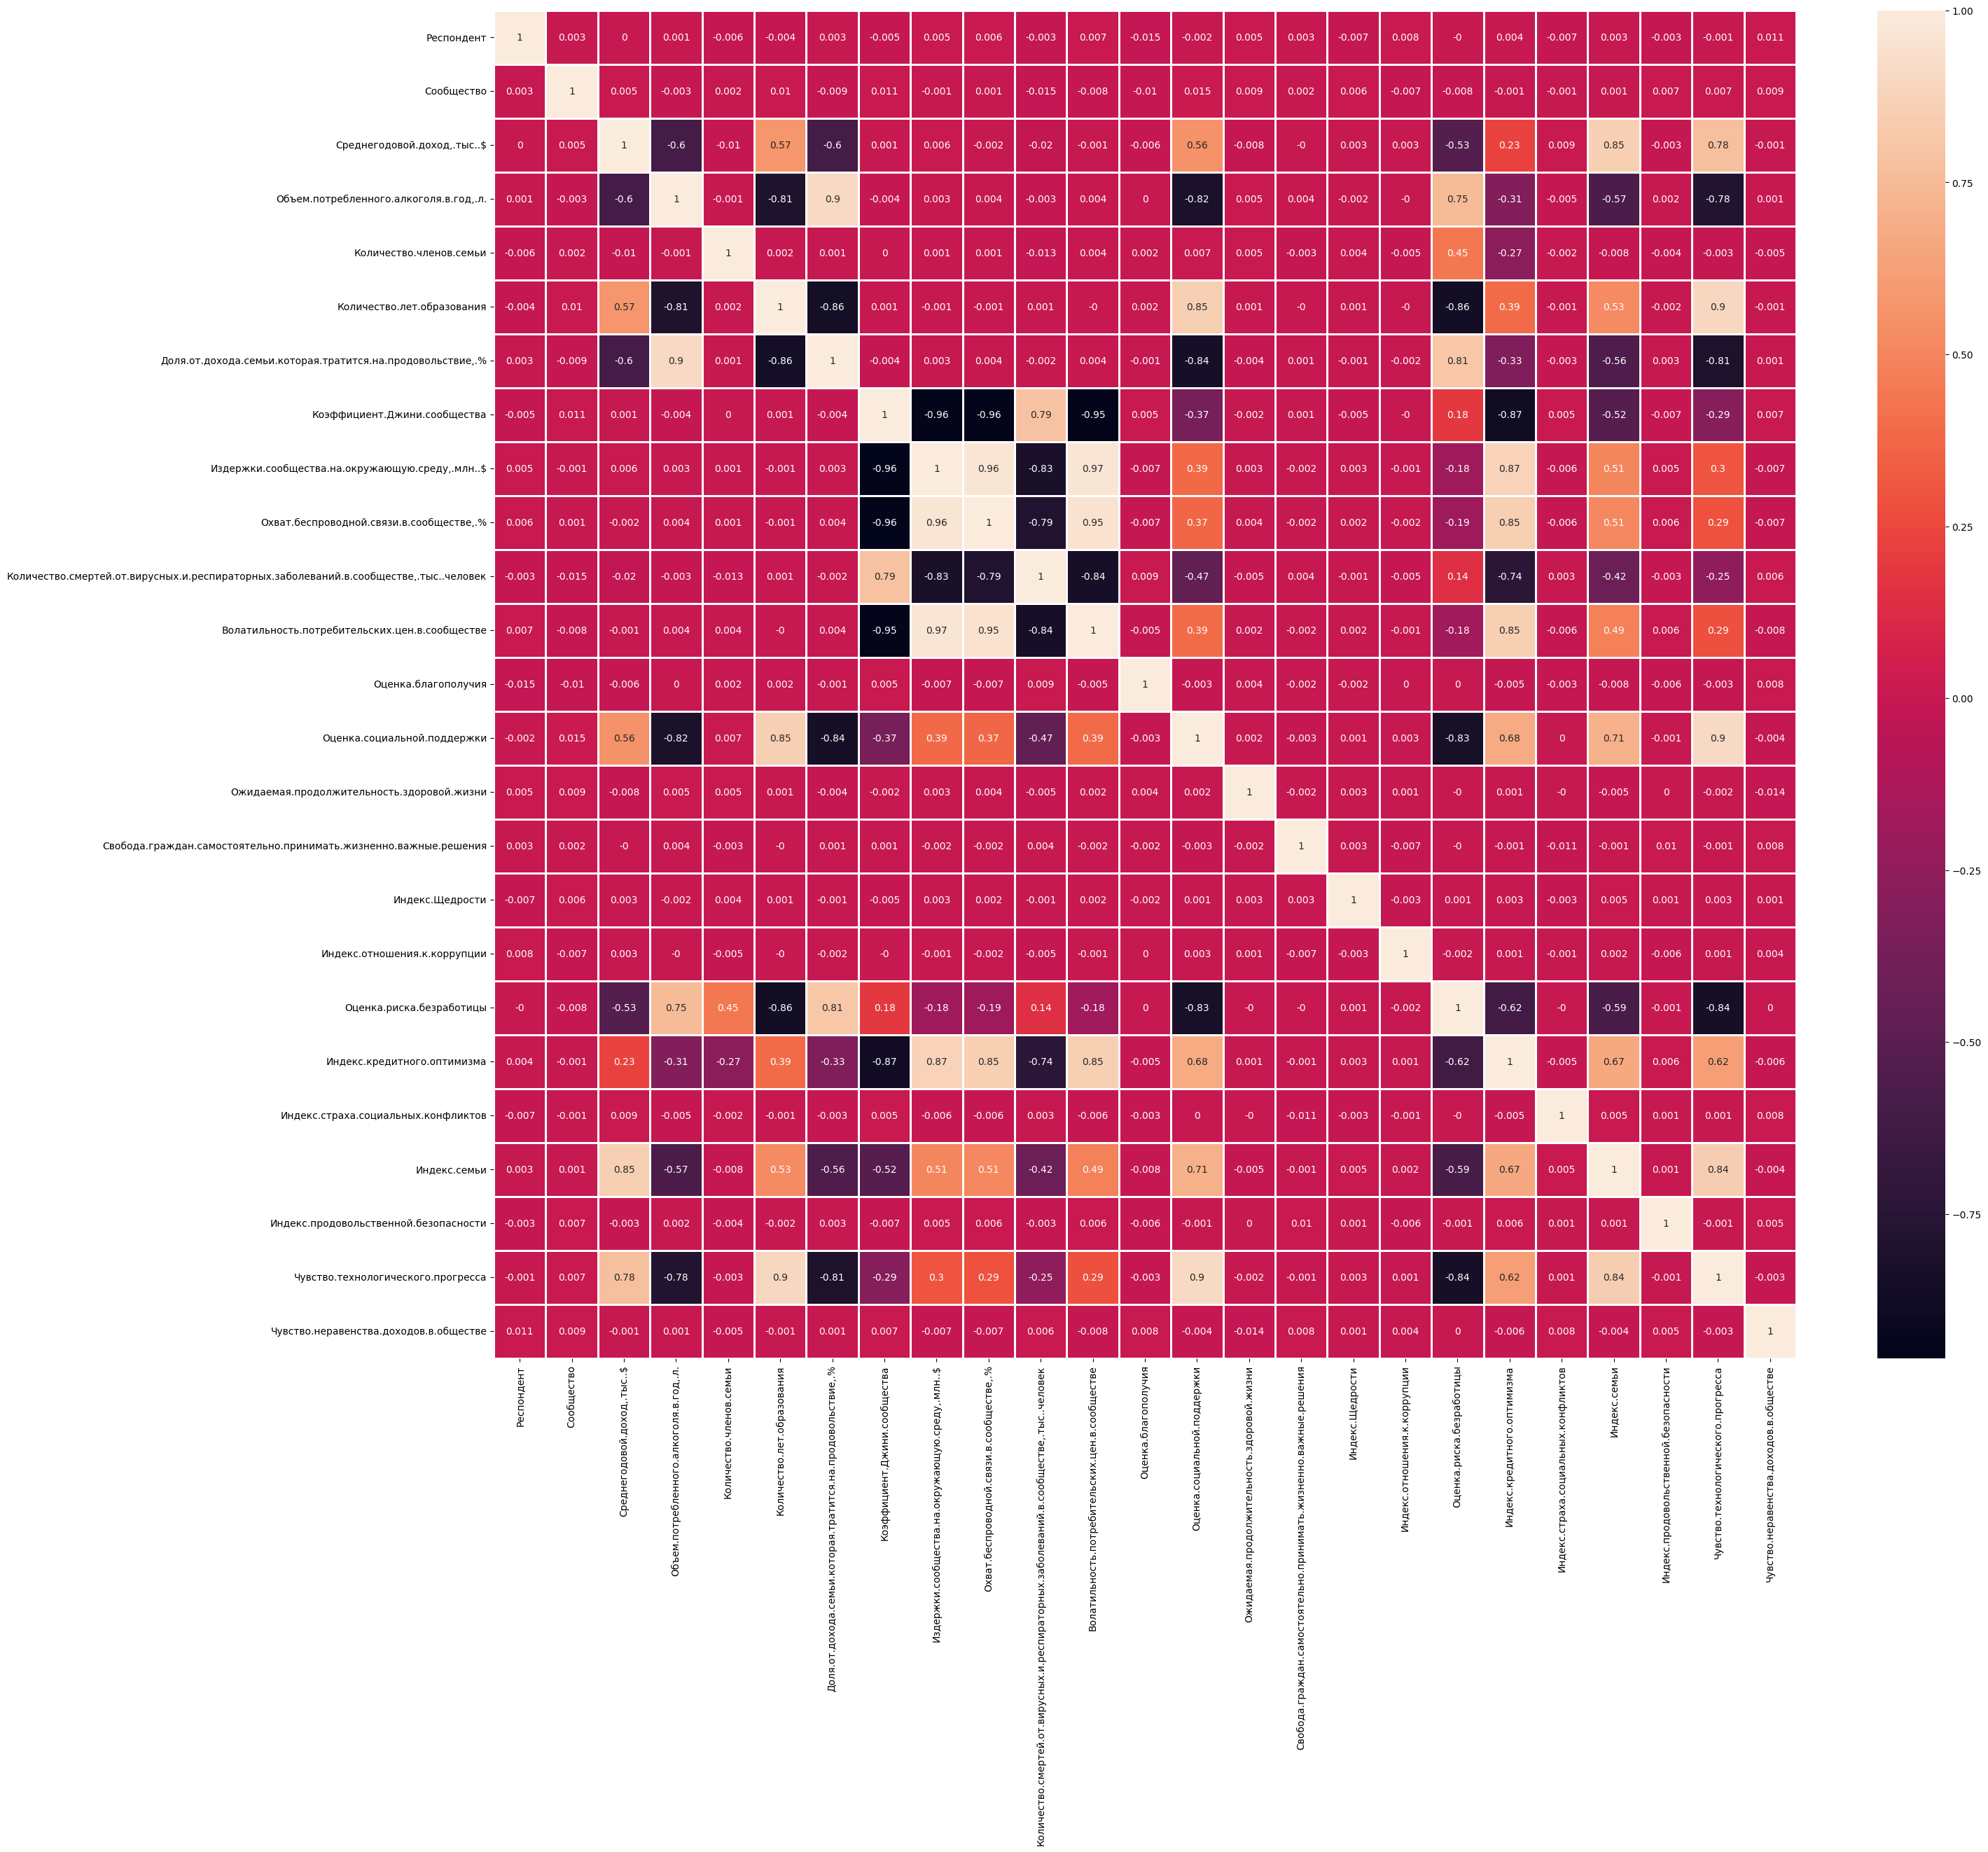
\includegraphics[width=\textwidth]{images/2.png}
	\end{center}
	\caption{Корреляционные зависимости между всеми признаками}
	\label{img:2}
\end{figure}

\begin{figure}
	\begin{center}
		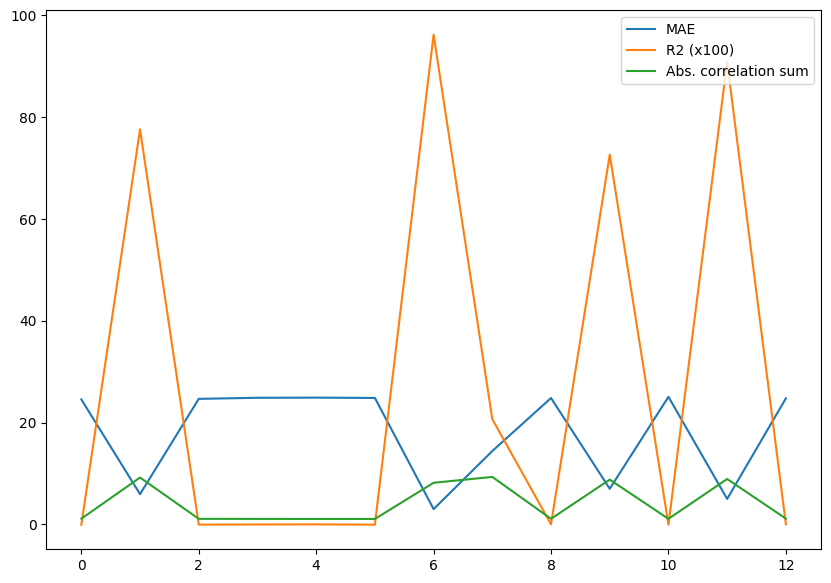
\includegraphics[width=\textwidth]{images/3.png}
	\end{center}
	\caption{Зависимость точности заполнения пропущенных значений признаков состояния от их корреляции с признаками причины}
	\label{img:3}
\end{figure}

\clearpage
